\chapter{単体モデル・統合モデルの性能評価}\label{ch:results}
本章では，10月15日完了のclean\_only実行143609を主系列とする\cite{localMainRun}．run hashは\texttt{da540f2d}，clean fitの識別子は\texttt{7560205f8feb}である．既存の検算記録では，全7条件で同じ540評価区間とclean fitを共有し，保存重みから6統合を再構成した結果が保存予測と一致している．本稿の表は保存CSVから抽出し，図は保存表・予測だけから描画した．モデルの再学習や新しい推論によって得た結果ではない．

まず問い\ref{rq:regression}に対して，全域回帰と雑音条件による差を示す．次に問い\ref{rq:onb}に対して，総判定，開始段階および検知到達熱流束を示し，両性能の利得と交換を対応づける．

\section{単体モデルの熱流束予測性能}
無雑音条件の全方式を表\ref{tab:clean}に示す．単体ではETの全域RMSEが28.40\,\kw{}，HGBが33.25\,\kw{}であり，CNN＋Transformer，AlexNet，RFとは差がある．34要約特徴を用いた追加2モデルは，この条件の全域回帰において有効な予測を与えた．ただし，これは入力表現と学習器を組み合わせた比較であるため，要約処理だけの優位を示す結果ではない．

\begin{table}[htbp]
\centering\small
\caption{無雑音における単体・統合の性能．RMSEの単位は\kw{}．近傍は30区間．}
\label{tab:clean}
% Generated from saved evidence; do not hand-edit.
\begin{tabular}{lrrrrr}
\toprule
方式 & RMSE & $R^2$ & 近傍RMSE & FN & FP \\
\midrule
RF (PCA+XGBRF) & 71.71 & 0.9296 & 113.59 & 45 & 1 \\
CNN+Transformer & 35.34 & 0.9829 & 38.71 & 35 & 1 \\
AlexNet & 39.88 & 0.9782 & 36.85 & 39 & 1 \\
HGB & 33.25 & 0.9849 & 26.15 & 21 & 0 \\
ET & 28.40 & 0.9890 & 9.73 & 19 & 2 \\
3-perf & 35.62 & 0.9826 & 46.46 & 44 & 1 \\
3-MSE & 34.07 & 0.9841 & 39.58 & 42 & 1 \\
3+HGB & 29.64 & 0.9880 & 24.91 & 24 & 0 \\
3+ET & 27.35 & 0.9898 & 13.37 & 26 & 1 \\
5-model & 27.80 & 0.9894 & 16.45 & 27 & 1 \\
5-equal & 32.78 & 0.9853 & 37.02 & 43 & 1 \\
\bottomrule
\end{tabular}

\end{table}

RFは，全域ではCNN系や追加2モデルより誤差が大きい．一方，雑音の影響や判定を含めて比較するには，この順位だけでは不十分である．単体である帯域や強度変化に反応しにくい場合でも，ONB未満を過大予測すれば誤報が多くなる可能性がある．単体の特徴は，回帰と判定の両方を参照して評価する．

\section{アンサンブルによる熱流束予測性能}
\subsection{元3から4・5モデルへの変化}
無雑音の元3 MSEのRMSEは34.07\,\kw{}，5モデル統合は27.80\,\kw{}であり，約18.40\%小さい．従来performanceの35.62\,\kw{}に対しても小さい．ET単体の28.40\,\kw{}も下回る．一方，元3＋ETの27.35\,\kw{}は5モデルの27.80\,\kw{}より小さい．従って，追加モデルを用いた利得は示されるが，HGBとETを両方加えた5モデルが無雑音で常に最良という結果ではない．

単体ETが元3＋ETより悪いことは，元3を残した統合がこの条件で補う部分を持つことを示す．ただし，元3内の三つ全てが不可欠という結論にはならない．同様に，5モデルが元3 MSEより良いことから，5というモデル数が最適であるとは言えない．構成，重み，入力の効果を一括して「モデル数の効果」と説明しない．

\subsection{予測値の分布}
図\ref{fig:scatter}に日別・端点条件での正解熱流束と予測値を示す．赤破線の縦線は記録段階のONB，横線は予測値に対する判定閾値である．高い熱流束側で予測が対角線に近い場合でも，縦線付近の点が横線より下にあれば開始段階を見逃す．このため，予測分布の全体像とONB近傍の閾値通過を分けて読む必要がある．

\begin{figure}[htbp]
\centering
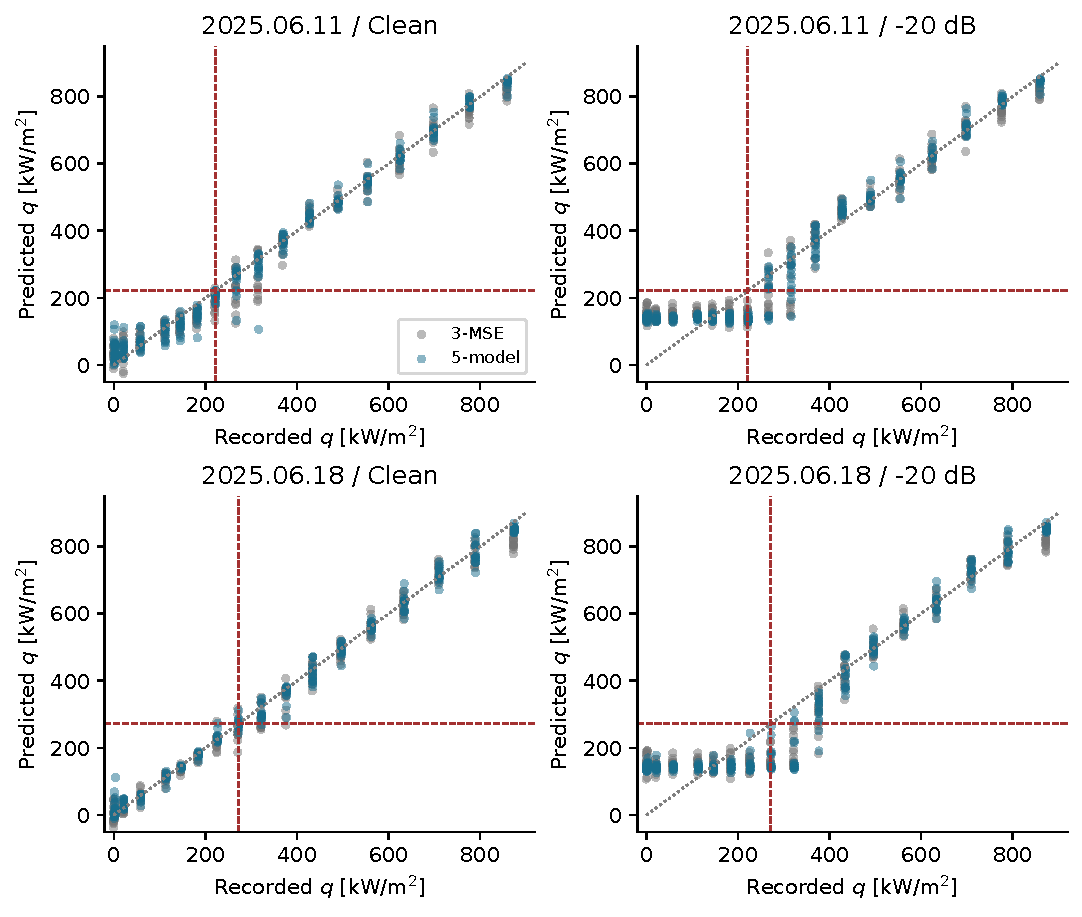
\includegraphics[width=0.98\textwidth]{prediction_scatter.pdf}
\caption{元3 MSEと5モデル統合の予測値．各日270評価区間を表示．同じ正解段階の点の重なりを軽減するため横座標に表示上のみ$\pm0.8$\,\kw{}を加えた．計算には元の正解を用いる．}
\label{fig:scatter}
\end{figure}

\section{雑音環境下における予測性能と耐性}
\subsection{雑音下の絶対性能}
全7条件のRMSEを表\ref{tab:noisermse}と図\ref{fig:noisermse}に示す．5モデル統合は元3 MSEおよび元3 performanceより全7条件で小さい．元3 MSEに対し，無雑音34.07から27.80\,\kw{}，$-20$\,dBで81.14から75.23\,\kw{}である．後者の低減率は約7.28\%である．この範囲では，追加2モデルを含む統合は雑音時の絶対誤差を改善する．

\begin{table}[htbp]
\centering\small
\caption{全7条件の集約RMSE [\kw{}]．基準SNRは各chunkの実現SNRとは異なる．}
\label{tab:noisermse}
% Generated from saved evidence; do not hand-edit.
\begin{tabular}{lrrrrrr}
\toprule
基準SNR & 3-perf & 3-MSE & 3+ET & 5-model & HGB & ET \\
\midrule
無雑音 & 35.62 & 34.07 & 27.35 & 27.80 & 33.25 & 28.40 \\
$0$ & 53.84 & 53.12 & 50.85 & 50.27 & 54.45 & 52.52 \\
$-4$ & 62.85 & 62.76 & 61.31 & 61.95 & 69.02 & 62.44 \\
$-8$ & 68.05 & 68.12 & 66.40 & 66.66 & 71.16 & 67.08 \\
$-12$ & 71.73 & 72.37 & 69.13 & 69.01 & 70.93 & 69.24 \\
$-16$ & 76.59 & 76.14 & 71.86 & 71.51 & 71.78 & 71.60 \\
$-20$ & 84.30 & 81.14 & 76.11 & 75.23 & 74.19 & 75.43 \\
\bottomrule
\end{tabular}

\end{table}
\begin{figure}[htbp]
\centering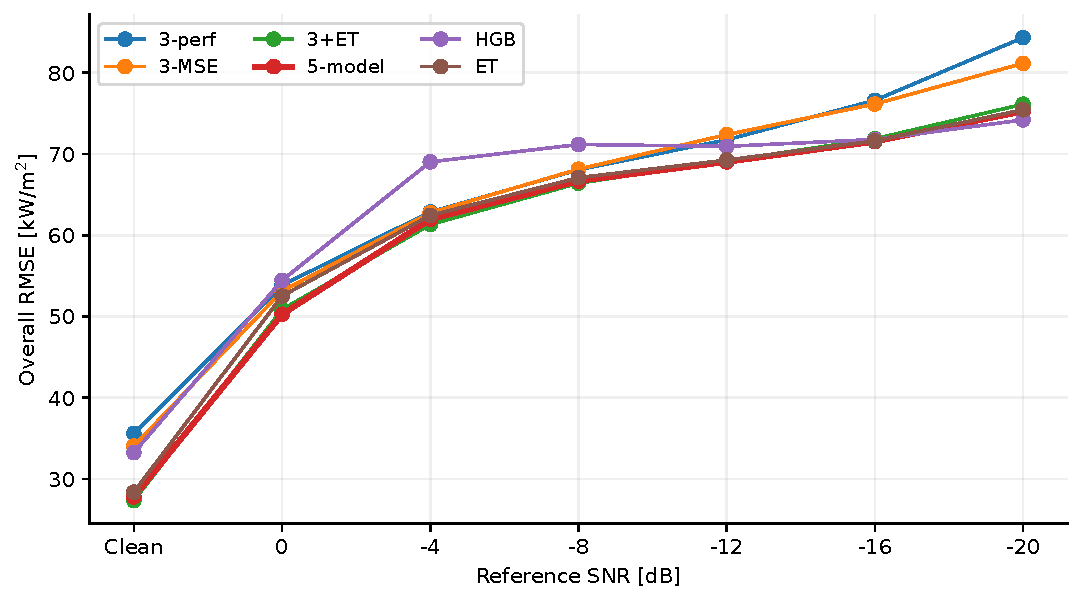
\includegraphics[width=0.97\textwidth]{noise_rmse.pdf}
\caption{固定学習済みモデルの全域RMSEと基準SNRの関係．同じ540区間の対応比較．}
\label{fig:noisermse}
\end{figure}

一方，$-20$\,dBではHGB単体が74.19\,\kw{}であり，5モデル75.23\,\kw{}より小さい．ET単体は75.43\,\kw{}で，5モデルとの差は小さい．元3＋ETに対しても，5モデルは無雑音，$-4$，$-8$\,dBでは悪化し，他の4条件では改善する．従って，統合の有効性は比較相手と雑音条件を指定して述べる必要がある．

評価後に各条件の最良単体を探すと，無雑音から$-16$\,dBまではET，$-20$\,dBではHGBとなる．これは事後的な記述比較であり，入力の真のSNRを知って最良単体を選択できる運用方式を実装した結果ではない．

\subsection{無雑音からの悪化量}
表\ref{tab:degradation}に無雑音から$-20$\,dBへのRMSE増加量を示す．元3 MSEは47.07\,\kw{}，5モデルは47.43\,\kw{}であり，5モデルの増加量は小さくなっていない．一方，元3 performanceの48.68\,\kw{}と比べれば5モデルの増加量は小さい．従って，「雑音下の誤差が改善した」という結論と，「悪化量を抑えた」という結論は比較基準に応じて分ける．
\begin{table}[htbp]
\centering
\caption{無雑音から基準SNR $-20$\,dBへの全域RMSE増加量 [\kw{}]．}
\label{tab:degradation}
% Generated from saved evidence; do not hand-edit.
\begin{tabular}{lrrr}
\toprule
方式 & 無雑音 & $-20$ dB & 増加量 \\
\midrule
3-perf & 35.62 & 84.30 & 48.68 \\
3-MSE & 34.07 & 81.14 & 47.07 \\
3+ET & 27.35 & 76.11 & 48.76 \\
5-model & 27.80 & 75.23 & 47.43 \\
HGB & 33.25 & 74.19 & 40.93 \\
ET & 28.40 & 75.43 & 47.03 \\
\bottomrule
\end{tabular}

\end{table}

元3 MSEに対する5モデルの絶対RMSE低減幅は，無雑音の約6.269から$-20$\,dBの約5.903\,\kw{}へ縮む．式\eqref{eq:gap_degradation}から，悪化量の低減は約$-0.366$\,\kw{}となる．保存表では付加雑音の全6条件で5のcleanからの増加量が元3 MSEより大きかった．元3 performanceに対しても，増加量が小さいのは$-20$\,dBの端点だけであり，他の5条件では小さくない．全域推定の絶対誤差低減は確認された成果であり，無雑音からの劣化量抑制はこの比較では支持されなかった結果である．

\section{沸騰開始判定性能}
\subsection{見逃しと誤報}
日別閾値を用いた判定を表\ref{tab:detection}と図\ref{fig:detection}に示す．5モデルのFN/FPは無雑音27/1，$-20$\,dBで52/0である．元3 MSEは42/1，65/0であり，5モデルは全7条件で総FNが少なく，FPは同数である．無雑音では元3の15件のFNを訂正し，新しいFNは0件であった．$-20$\,dBでも13件を訂正し，新FNは0件である\cite{localMainRun}．

\begin{table}[htbp]
\centering\small
\caption{日別閾値を用いたONB判定．全体の正例315，負例225区間．}
\label{tab:detection}
% Generated from saved evidence; do not hand-edit.
\begin{tabular}{lrrrr}
\toprule
基準SNR & 3-MSE FN/FP & 3+ET FN/FP & 5-model FN/FP & 5 Recall [\%] \\
\midrule
無雑音 & 42 / 1 & 26 / 1 & 27 / 1 & 91.43 \\
$0$ & 45 / 0 & 44 / 1 & 44 / 0 & 86.03 \\
$-4$ & 52 / 0 & 45 / 1 & 45 / 0 & 85.71 \\
$-8$ & 57 / 0 & 46 / 0 & 47 / 0 & 85.08 \\
$-12$ & 60 / 0 & 48 / 0 & 48 / 0 & 84.76 \\
$-16$ & 65 / 0 & 51 / 0 & 50 / 0 & 84.13 \\
$-20$ & 65 / 0 & 52 / 0 & 52 / 0 & 83.49 \\
\bottomrule
\end{tabular}

\end{table}
\begin{figure}[htbp]
\centering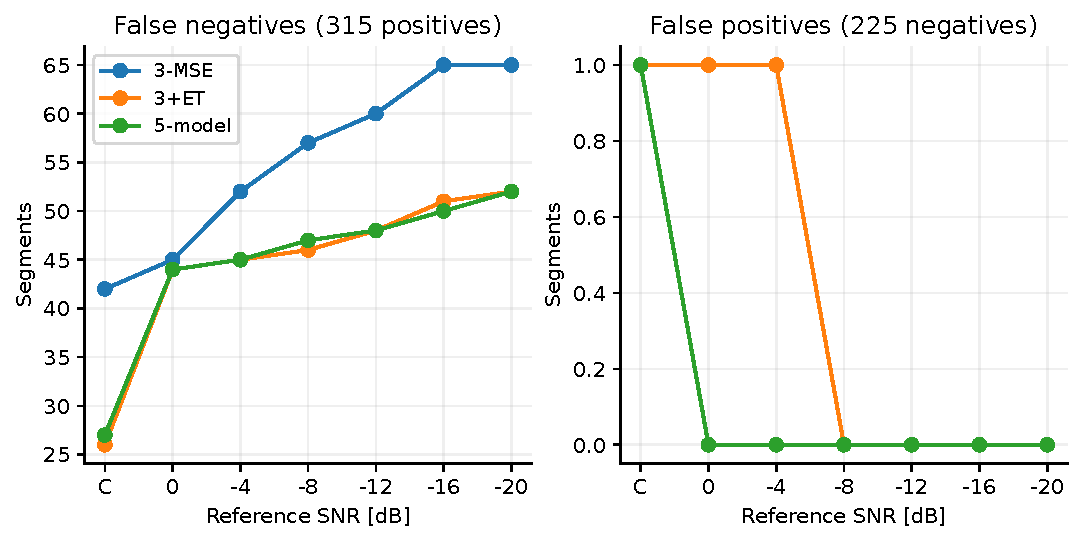
\includegraphics[width=0.98\textwidth]{detection_errors.pdf}
\caption{雑音条件別のFNとFP．同じ熱流束予測から回帰と判定を評価する．}
\label{fig:detection}
\end{figure}

単体ETを基準にすると，無雑音では5モデルのFNは19から27へ増える．標本別にはETのFNを2件訂正する一方，ETで陽性だった10件を新たにFNとした．従って，平均化は良い判定を保存する処理ではない．ある単体の陽性が他の予測と混ざることで，閾値未満へ戻る場合がある．

\begin{table}[htbp]
\centering\small
\caption{基準SNR $-20$\,dBの単体・統合性能．RMSEの単位は\kw{}．}
\label{tab:noisy}
% Generated from saved evidence; do not hand-edit.
\begin{tabular}{lrrrrr}
\toprule
方式 & RMSE & $R^2$ & 近傍RMSE & FN & FP \\
\midrule
RF (PCA+XGBRF) & 151.28 & 0.6865 & 61.98 & 0 & 217 \\
CNN+Transformer & 81.62 & 0.9088 & 96.37 & 68 & 0 \\
AlexNet & 81.66 & 0.9087 & 124.94 & 65 & 0 \\
HGB & 74.19 & 0.9246 & 107.28 & 49 & 0 \\
ET & 75.43 & 0.9221 & 100.34 & 50 & 1 \\
3-perf & 84.30 & 0.9027 & 79.16 & 62 & 0 \\
3-MSE & 81.14 & 0.9098 & 93.92 & 65 & 0 \\
3+HGB & 74.95 & 0.9230 & 100.74 & 55 & 0 \\
3+ET & 76.11 & 0.9207 & 98.38 & 52 & 0 \\
5-model & 75.23 & 0.9225 & 99.32 & 52 & 0 \\
5-equal & 82.42 & 0.9070 & 74.24 & 52 & 0 \\
\bottomrule
\end{tabular}

\end{table}

表\ref{tab:noisy}ではRF単体のFNが0である一方，FPは217である．これは負例225区間の大部分を誤報する状態であり，FNの少なさだけから早期検知に適すると判断できない．局所誤差や$q_{100}$も同様に，誤報との組合せで解釈する．

\subsection{日別の検知到達熱流束}
表\ref{tab:q100}と図\ref{fig:q100}に$q_{100}$を示す．6月18日の無雑音では元3 MSEの434.02\,\kw{}から5モデルの376.32\,\kw{}へ低下するが，元3＋ETは322.11\,\kw{}である．6月11日は元3 MSE，元3＋ET，5モデルとも368.98\,\kw{}であり，総FNが減っても到達段階は変わらない．
\begin{table}[htbp]
\centering\small
\caption{日別の検知到達熱流束$q_{100}$とONBからの差$g_{100}$ [\kw{}]．}
\label{tab:q100}
% Generated from saved evidence; do not hand-edit.
\begin{tabular}{lrrrrr}
\toprule
日・条件 & ONB & 3-MSE & 3+ET & 5-model & $g_{100}$ (5) \\
\midrule
06.11 無雑音 & 221.51 & 368.98 & 368.98 & 368.98 & 147.47 \\
06.11 $-20$ & 221.51 & 368.98 & 368.98 & 368.98 & 147.47 \\
06.18 無雑音 & 271.68 & 434.02 & 322.11 & 376.32 & 104.64 \\
06.18 $-20$ & 271.68 & 434.02 & 434.02 & 434.02 & 162.34 \\
\bottomrule
\end{tabular}

\end{table}
\begin{figure}[htbp]
\centering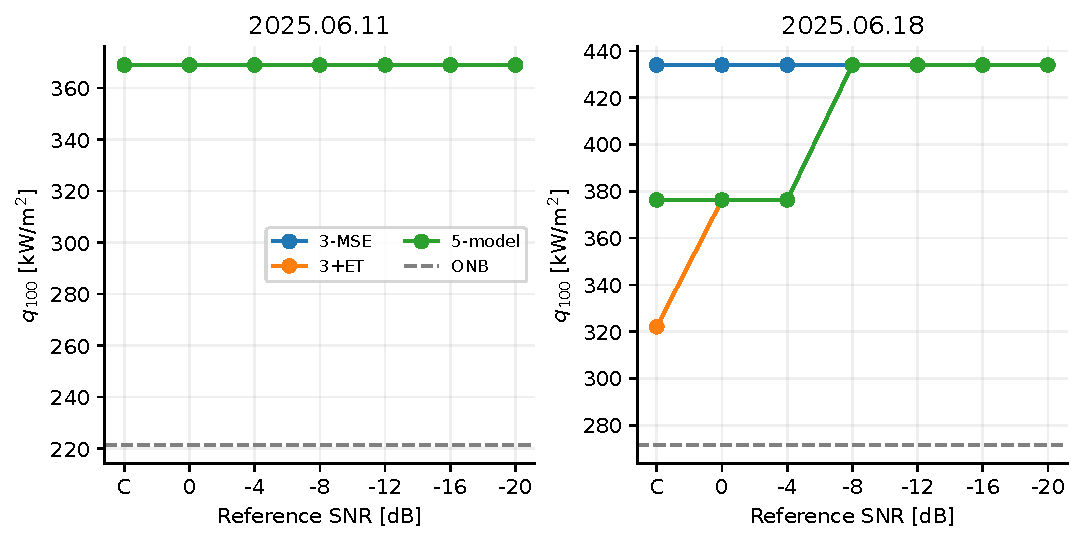
\includegraphics[width=0.98\textwidth]{q100.pdf}
\caption{日別$q_{100}$の雑音条件依存．破線は各日の採用ONB値．}
\label{fig:q100}
\end{figure}

$q_{100}$は最後に残るFNの段階へ強く依存する．他の段階で多数のFNを訂正しても，その最終段階に1件残れば値が変わらない．逆に1件の訂正で一段前進する場合もある．従って，FN総数の改善と$q_{100}$の改善は矛盾する指標ではなく，判定の異なる側面を表している．

\section{ONB近傍における予測性能}
5モデルの近傍RMSEは，無雑音では元3 MSEの39.58から16.45\,\kw{}へ低下する．一方，$-20$\,dBでは93.92から99.32\,\kw{}へ増えた．全域RMSEの全7条件での改善は，ONB近傍まで一律に改善することを意味しない．

さらに，記録上ONB段階の30区間に対する検知を表\ref{tab:onset}に示す．5モデルは無雑音で8区間を検知し，22区間を見逃す．$-20$\,dBでは全30区間を見逃す．全ONB以上315区間に対するRecallは無雑音91.43\%，$-20$\,dBで83.49\%であるが，開始段階に限定した割合はそれぞれ26.67\%，0\%となる．母数と対象段階を変えると見える結論が異なる．

\begin{table}[htbp]
\centering\small
\caption{5モデル統合の記録上ONB段階における判定．2 WAVから各15評価区間，計30区間．}
\label{tab:onset}
% Generated from saved evidence; do not hand-edit.
\begin{tabular}{lrrrr}
\toprule
基準SNR & 記録上ONB段階 & 検知 & 見逃し & 検知割合 [\%] \\
\midrule
無雑音 & 30 & 8 & 22 & 26.67 \\
$0$ & 30 & 2 & 28 & 6.67 \\
$-4$ & 30 & 2 & 28 & 6.67 \\
$-8$ & 30 & 2 & 28 & 6.67 \\
$-12$ & 30 & 1 & 29 & 3.33 \\
$-16$ & 30 & 0 & 30 & 0.00 \\
$-20$ & 30 & 0 & 30 & 0.00 \\
\bottomrule
\end{tabular}

\end{table}

この30区間は独立した30回のONB発生実験ではない．二つの段階録音から抽出された評価区間の判定であり，区間に真の気泡発生秒のラベルがあるわけでもない．この範囲でも，開始段階の十分な検知を達成したという結論は支持されない．

近傍RMSEには非単調な変化もある．5モデルでは$-12$\,dBの113.32から$-20$\,dBの99.32\,\kw{}へ小さくなる一方，総FNは48から52へ増え，ONB段階の見逃しも29から30へ増える．平均予測が上方へ動いて誤差が小さくなっても，閾値を超えない限り判定は訂正されない．局所回帰誤差の回復を，ONB検知の回復と同義には扱わない．

\section{熱流束予測精度と沸騰開始判定性能の関係}
本章の結果は，熱流束回帰とONB判定が同じ予測を用いながら，異なる評価を必要とすることを示す．元3 MSEから5モデルへの変更で，全域RMSEと総FNは改善した．しかし，無雑音のET4に対する優位，$-20$\,dBのHGBに対する優位，ONB近傍と最初のONB段階の十分な検知は得られていない．

全域MSEは，全区間の二乗誤差を小さくする指標である．ONB判定は，予測が閾値のどちらに位置するかで決まる．そのため，近傍の小さな過小予測が検知上重大でも，高熱流束側の大きな誤差低減によって全域指標が改善することはあり得る．本研究ではこの関係を実際の保存予測で確認した．

問い\ref{rq:regression}に対しては，対象の全7条件で元3 MSEより全域推定誤差を低減したと回答できる．問い\ref{rq:onb}に対しては，全7条件で総FNを減らしFPを維持した一方，開始段階・近傍・日別$q_{100}$への利得は限定的であったと回答できる．全域推定と総判定は独立した主要成果として述べ，開始段階の限界も同じ回答の中へ残す．次章では問い\ref{rq:explanation}に対して，どの領域・誤差群が変わり，どの入力と制約が関係するかを考察する．
